\documentclass[../main]{subfiles}
\begin{document}
\chapter{percolationと振動数同期}
\label{chap:percolation}
\section{問題設定及び数値実験}
\ref{sec:method-3body-settting}節と同様にERモデル (Erd\H{o}s–R\'{e}nyi model) $\Gamma_{n,m}$ において,枝の本数$m$を変化することでモデルの構造を変化させることを振動子ネットワークで考える.
すなわち,$n$体の振動子ネットワークにおいて$m=0$から$m=n(n-1)/2$まで枝の本数を連続的に変化させる.
このとき,構造の変化に伴い同期状態が変化することが考えられる.\\
以下,簡単のため固有振動数の分布として$\omega_\pm$の二項分布$\operatorname{Bin}(n,p)$を用いることとする.\\
$m=0$から$m=n(n-1)/2$まで枝の本数を連続的に変化させることを1試行とし,$M(>1)$回行い,以下の特徴量の平均を求める.
\begin{itemize}
    \item 
    同じ実効振動数を持つ集団のサイズの最大値$L$.ただし,実効振動数差が$\Delta\ll 1$の振動子を同一の振動数とみなすこととする.
    \item
    オーダーパラメータ$R$
    \begin{align*}
        R\mathrm{e}^{\imag \psi}:=\frac{1}{n}\sum_{j=1}^n\mathrm{e}^{\imag \theta_j}    
    \end{align*}
\end{itemize}
固有振動数の分布として$\pm 1$の二項分布を用いた$n=50$個の振動子に対し,枝の数を$0$から$1225$本まで変化させた試行を$M=100$回行い平均したものを図\ref{fig:edge-strict400}に示す.
\begin{figure}[H]
\centering
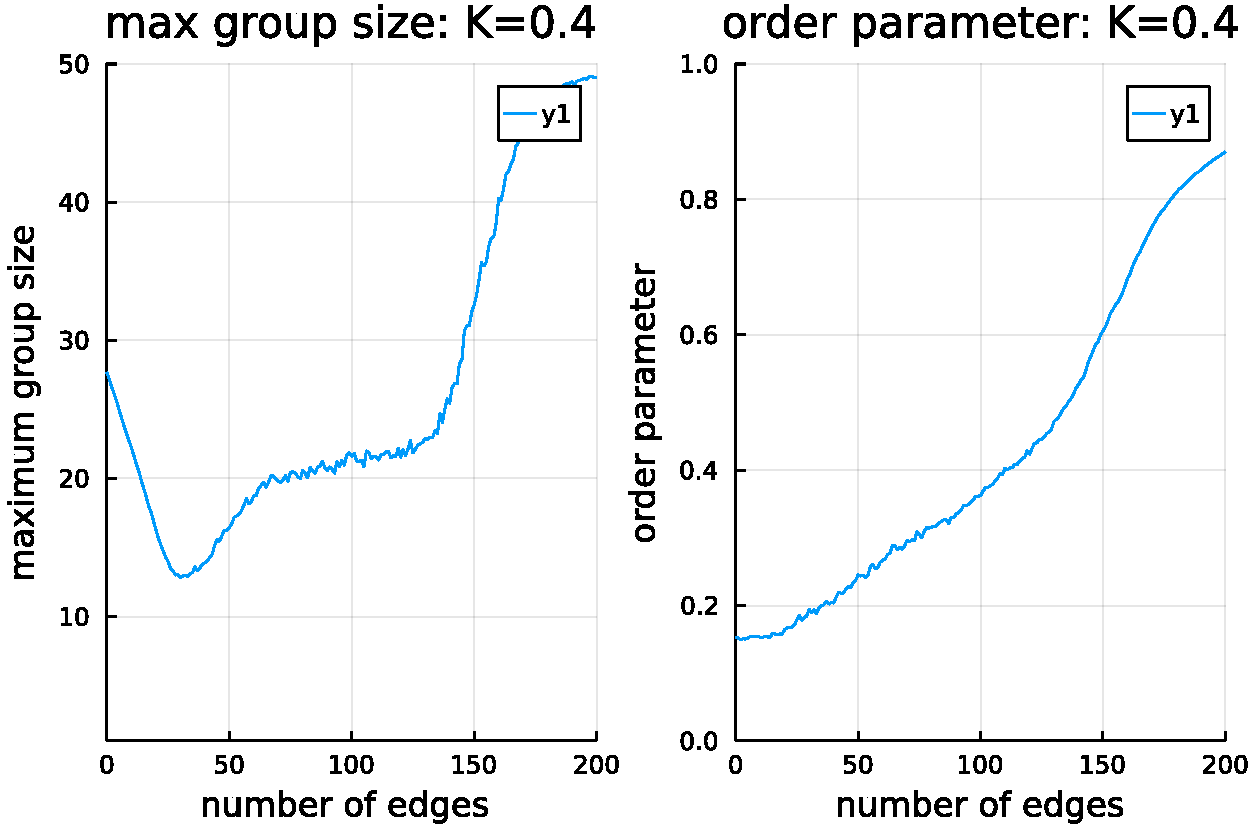
\includegraphics[width=105mm]{images/edge-finite-strict400.pdf}
\centering
\caption{$n=50,K=0.4$のときの枝の本数と振動数によるクラスタの最大数(左)とオーダーパラメータ(右)の関係.\\
左図では,$m=0$から$m=30$付近まで線形に減少し極小値を取り,その後増加し$m=70$付近で概ね停滞する.
そして,$m=125$付近から増加に転じ最大値に収束する.\\
右図では,$m=0$から緩やかに増加し$m=30,70$付近で変曲点を向かえながら$m=125$付近で最大値に収束する.
}
\label{fig:edge-strict400}
\end{figure}
4つの同期状態に分かれている.それぞれの境界に相当する枝の臨界本数を$m_1,m_2,m_3$とすると以下のようにまとめられる.\\
$0\leq m<m_1$では最大集団のサイズ$L$が線形に減少する (Phase 1) .
$m_1\leq m_2$では最大集団のサイズ$L$が増加し (Phase 2) ,$m_2\leq m_3$では最大集団のサイズ$L$がほぼ変化しない (Phase 3) .
$m=m_3$付近で最大集団のサイズ$L$が大きく増加し$L=n$となり,同時にオーダーパラメータが増加し$R=1$となる.$m\gtrsim m_3$では,$L=n,R=1$で変化しない (Phase 4) .
\section{同期状態の定性的解釈}
それぞれの同期状態は定性的に以下のように理解できる.
\renewcommand{\labelenumi}{Phase \theenumi}
\begin{enumerate}
    \item 固有振動数$\omega_\pm$の孤立した頂点が主な振動数となる.
    枝が1本増えるごとに高い確率で孤立した頂点をつなぐため,固有振動数$\omega_\pm$を実効振動数にもつ頂点数は平均$p$本減少する.
    よって,$L(m)=np-mp$となる.
    \item \label{phase-2}最大連結集団に属する振動子のもつ実効振動数が主な振動数となる.
    \item Phase \ref{phase-2}と同様に,最大連結集団に属する振動子のもつ実効振動数が主な振動数となるが,同じ固有振動数を持つ振動子同士がほとんど同期し$L$が停滞する.
    \item 異なる振動子同士が同期し,全体が同期する.
\end{enumerate}
\section{臨界本数}
\subsection{最大サイズ$L$の極小値を与える枝の本数$m_1$}
数値実験によると$K$に依らない.
\subsection{最大サイズ$L$が上がり留まる枝の本数$m_2$}
数値実験によると$K$に依らない.
\subsection{最大サイズ$L$,オーダーパラメータ$R$が大きく変化する枝の本数$m_3$}
枝の本数が頂点数に比べ十分多いので,固有振動数$\omega_\pm$を持つ2種類の振動子として平均場近似することができる.
\begin{align*}
    \dot{\phi}_+&=\omega_++\frac{m}{n}K\sin(\phi_--\phi_+)\\
    \dot{\phi}_-&=\omega_-+\frac{m}{n}K\sin(\phi_+-\phi_-)
\end{align*}
この同期条件は
\begin{align*}
    K\geq \frac{(\omega_+-\omega_-)n}{2m}
\end{align*}
よって,
\begin{align*}
    m_3=\frac{(\omega_+-\omega_-)n}{2K}
\end{align*}
となる.
\end{document}